\documentclass[final]{beamer}
% beamer 3.10: do NOT use option hyperref={pdfpagelabels=false} !
% \documentclass[final,hyperref={pdfpagelabels=false}]{beamer} 
% beamer 3.07: get rid of beamer warnings

\mode<presentation> {  
%% check http://www-i6.informatik.rwth-aachen.de/~dreuw/latexbeamerposter.php for examples
  \usetheme{Durham} %% This points to the theme cooked up by the final year tutor
}


\usepackage[english]{babel} 
\usepackage[latin1]{inputenc}
\usepackage{amsmath,amsthm, amssymb, latexsym}

  \usefonttheme[onlymath]{serif}
  \boldmath
  \usepackage[orientation=portrait,size=a3,scale=1.4,debug]{beamerposter}                       

  % e.g. for DIN-A0 poster
  % \usepackage[orientation=portrait,size=a1,scale=1.4,grid,debug]{beamerposter}
  % e.g. for DIN-A1 poster, with optional grid and debug output
  % \usepackage[size=custom,width=200,height=120,scale=2,debug]{beamerposter} % e.g. for custom size poster
  % \usepackage[orientation=portrait,size=a0,scale=1.0,printer=rwth-glossy-uv.df]{beamerposter}
  % e.g. for DIN-A0 poster with rwth-glossy-uv printer check ...
  %

  \title[Final Year Project Poster]{Cloud-based RAW Image Editing}
  \author[R Collins]{Ryan Collins}
  \institute[Durham]{Department of Computer Science, Durham University}
  \date{\today}

  \begin{document}
  \begin{frame}{} 

  \vfill
    \begin{columns}[t]
      \begin{column}{.48\linewidth}
        \begin{block}{Introduction}

          This poster describes the design and implementation of
          a Cloud-based system for processing and editing RAW images.
          Previous RAW image editing software is designed for native
          use, and most of the current software available is proprietary.
          This paper shows the design and implementation of a system
          that's not proprietary, and allows for editing of RAW images
          through our Cloud-based RAW image editing service.

        \end{block}

       

        \begin{block}{Design System and GA}
          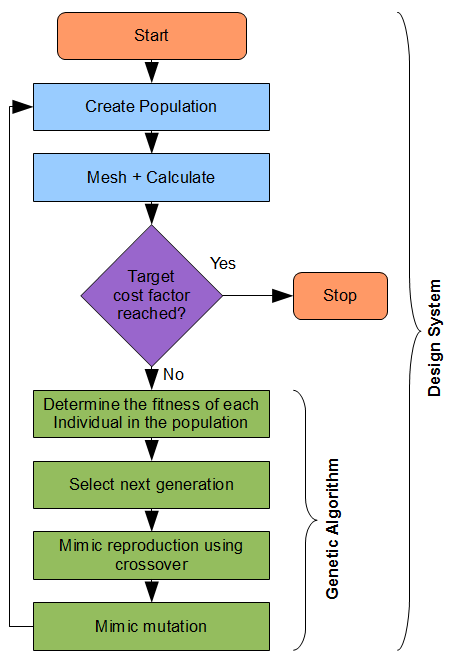
\includegraphics[width=\columnwidth]{DesignSystemandGA}  
        \end{block}
      \end{column}


      \begin{column}{.48\linewidth}
        \begin{block}{Some Example Equations}
          \begin{itemize}
          \item A fourier series $f\left(t\right)=a_{0} +
            \sum^{\infty}_{n=1} \left(a_{n} \cos \frac{n \pi t}{L} +
              b_{n} \sin \frac{n \pi t}{L}\right)$
        \item Secondary energy coefficient $C_{SKE} = \frac{U^2_{sec}
            + U^2_r}{U^2_{ups}}$
        \item A cost function $f_{cost} = f_{C_{SKE}}+f_{yaw} +
          f_{mass}$
          \end{itemize}
        \end{block}

        \begin{block}{A Sample Figure}
          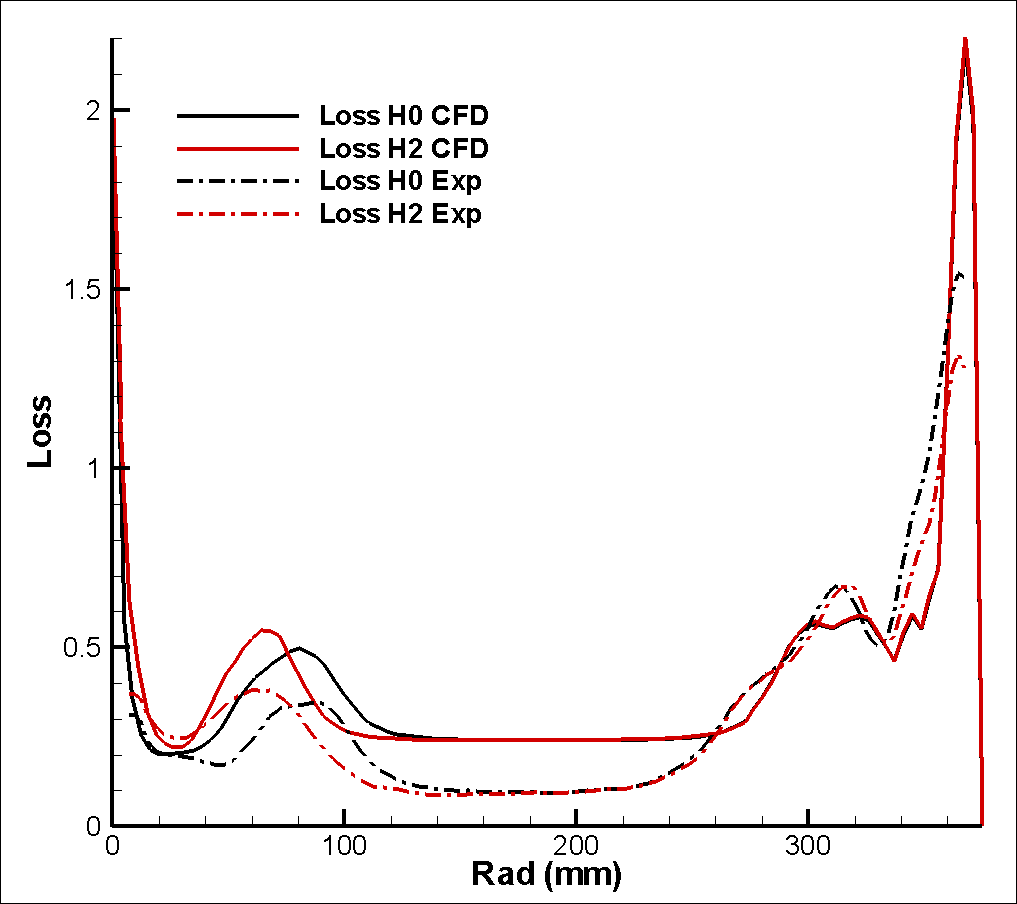
\includegraphics[width=\columnwidth]{pa_loss}  
        \end{block}

 \begin{block}{Some Sample Text}

          Tip leakage flow is caused by fluid flow through the tip gap
          of an un-shrouded blade driven by a pressure gradient
          between pressure side and suction side of a blade. The flow
          is quite complex but the main feature is the flow over the
          tip forming a streamwise vortex. The cross passage flow also
          separates from the endwall and rolls up into a passage
          vortex. From the blade mid-span toward the tip gap endwall
          the tip leakage vortex is usually the dominant structure and
          has an opposite rotation sense compared to passage
          vortex. The relations between the circulation and size of
          the two structures depend among others mainly on tip gap
          size and flow turning angle.

        \end{block}

      \end{column}
    \end{columns}

  \vfill
    \begin{block}{\large This shows different font sizes you can use}
      \centering
      {\tiny tiny}\par
      {\scriptsize scriptsize}\par
      {\footnotesize footnotesize}\par
      {\normalsize normalsize}\par
      {\large large}\par
      {\Large Large}\par
      {\LARGE LARGE}\par
      {\veryHuge VeryHuge}\par
      {\VeryHuge VeryHuge}\par
      {\VERYHuge VERYHuge}\par
    \end{block}
    \vfill

  \end{frame}
\end{document}


